\documentclass{article}

\usepackage[utf8]{inputenc}
\usepackage{longtable}
\usepackage{authblk}
\usepackage{adjustbox}
\usepackage{natbib}
\usepackage{graphicx}
\graphicspath{ {Imagenes/} }
\usepackage{array}
\usepackage{tabu}
\usepackage{multirow}
\usepackage{amsmath}
\usepackage{adjustbox}


\title{Índices de Desarrollo: Correlación con la Población Colombiana}
% autores
\renewcommand\Authand{, y }
\author[1]{\normalsize Juan Sebastián Cortázar}
\author[2]{\normalsize María Alejandra Restrepo}
\author[3]{\normalsize Juan Camilo Rueda}


\affil[1,2,3]{\small  Universidad de los Andes\\
\texttt{{js.cortazar533,ma.restrepot,jc.rueda169}@uniandes.edu.col}}



\date{7 de Julio de 2018}

%%%%

\usepackage{Sweave}
\begin{document}
\Sconcordance{concordance:ProyFMerge.tex:ProyFMerge.Rnw:%
1 33 1 1 0 76 1}


\maketitle


\begin{abstract}

En este trabajo se muestra el **Índice de Desarrollo Humano** (IDH) de Colombia por departamento, donde a través de estadística poblacional se observa el nivel de educación, nivel de salud e ingresos per cápita de los distintos departamentos para poder determinar los departamentos más vulnerables y los que tienen un mejor índice. Adicional, se identifica una correlación entre la población y el IDH, por lo cual se hace una regresión entre el IDH y las poblaciones de cabecera por departamento y el total de población de cada departamento con el IDH.

\end{abstract}

\section*{Introduccio´n}

El I´ndice de Desarrollo Humano es una medida utilizada para determinar el crecimiento y el desarrollo de las zonas y los pai´ses teniendo no solo en cuenta el crecimiento econo´mico. Este i´ndice busca medir no solo los PIB per ca´pita de las personas, sino que busca entender el acceso a salud y a la educacio´n que determinan la posibilidad de crecimiento de las sociedades y sus capacidades de generar unas mejores condiciones de vida. 
El valor del IDH es la media geome´trica entre los i´ndices normalizados de las tres dimensiones (Salud, Educacio´n y Nivel de Vida) como se muestra en la imagen \ref{IDH} a continuacio´n. 


%imagen de calculo del IDH
\begin{figure}[h]
\centering
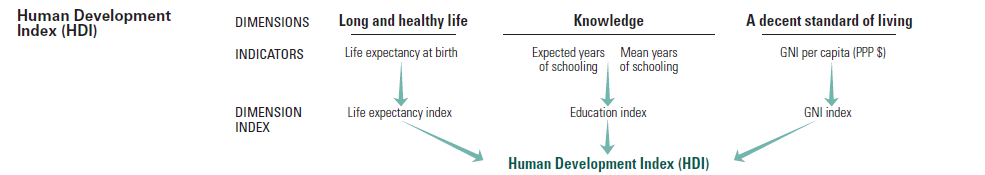
\includegraphics{hdiCalc}
\label {IDH}
\end{figure}

Para el cálculo de cada uno de los índices se tienen unos límites inferiores y superiores que en conjunto con los valores del sector (ya sea país o departamento) generan cada uno de los índices. En la tabla \ref{Tabla 1:} se puede ver lo siguiente.

%tabla boundary values

\begin{table}[h!]
\centering
  \begin{tabular}{l c c c}
  \hline
  Dimensiones & Indicador & Min & Max \\ [0.25ex]
  \hline \hline
  Salud & Expectancia de Vida (an~os) & 20 & 85 \\
  \multirow{2}{*}{Educacio´n} & Escolaridad Adultos & 0 & 18 \\ 
   & Esperanza educativa nin~os & 0 & 15 \\
  Nivel de Vida  & PIB per Capita (USD ctes 2011) & 100 & 75,000 \\
  \hline
  \end{tabular}
 \caption {Rango de Dimensiones IDH}
  \label{Tabla 1:}
\end {table} 

La variable Salud se genera a trave´s de un i´ndice compuesto que refleja condiciones de salud en los hogares: proteccio´n de salud, a trave´s del IGSS o de un seguro, nu´mero de personas por dormitorio, tipo de acceso a agua y saneamiento y tipo de piso en la vivienda. Todos estos factores influencian la expectantica de vida y se calculan de la siguiente manera.

\[ Salud=\frac{LE-20} {85-20} \]

Donde $LE = Expectativa de Vida$
La variable Educacio´n es un indicador compuesto que incluye la escolaridad alcanzada por adultos mayores de 25 an~os y la esperanza educativa en nin~os. En el primer indicador se mide la tasa de alfabetizacio´n de adultos en el segundo se mide la tasa bruta combinada de matriculacio´n en educacio´n primara, secundario y superior, asi´ como los an~os de duracio´n de la educacio´n obligatoria. El ca´lculo del i´ndice de educacio´n se define de la siguiente manera
\[Educacio´n= \frac{EA + EN} {2} \]
Donde
\[EA= \frac{Prom de an~os de educacio´n adultos} {18}  \]
\[EN= \frac{Prom de an~os de educacio´n nin~os} {15}  \]

La variable del nivel de vida mide el PIB per ca´pita de una zona o pai´s teniendo en cuenta un mi´nimo esperado y un maximo. La formula es la siguiente

\[Nivel de Vida = \frac {Ln(PIBx) – Ln (100)} {Ln(75,000)-Ln(100)} \]





Comencemos viendo que hay en la seccio´n \ref{univariada} en la pa´gina \pageref{univariada}.

\clearpage






\section{Exploración Univariada}\label{univariada}


En esta sección nos interesa explorar cada indice (IDH), para esto se realizan varias estadisticas con la información obtenida. En primer lugar, se evalua el numero de datos y la mediana de cada uno de los tipos de población.En la tabla ref{stats} en la página \pageref{stats}.





% Table created by stargazer v.5.2.2 by Marek Hlavac, Harvard University. E-mail: hlavac at fas.harvard.edu
% Date and time: mar, jul 03, 2018 - 05:49:47 p.m.
\begin{table}[!htbp] \centering 
  \caption{Medidas estadísticas} 
  \label{stats} 
\begin{tabular}{@{\extracolsep{5pt}}lcc} 
\\[-1.8ex]\hline 
\hline \\[-1.8ex] 
Statistic & \multicolumn{1}{c}{N} & \multicolumn{1}{c}{Median} \\ 
\hline \\[-1.8ex] 
cabecera & 32 & 717,197 \\ 
resto & 32 & 268,111.5 \\ 
\hline \\[-1.8ex] 
\end{tabular} 
\end{table} 
Para resaltar lo anterior, tenemos la Figura \ref{histograma} en la página \pageref{histograma}. 


%%%%% figure
\begin{figure}[h]
\centering
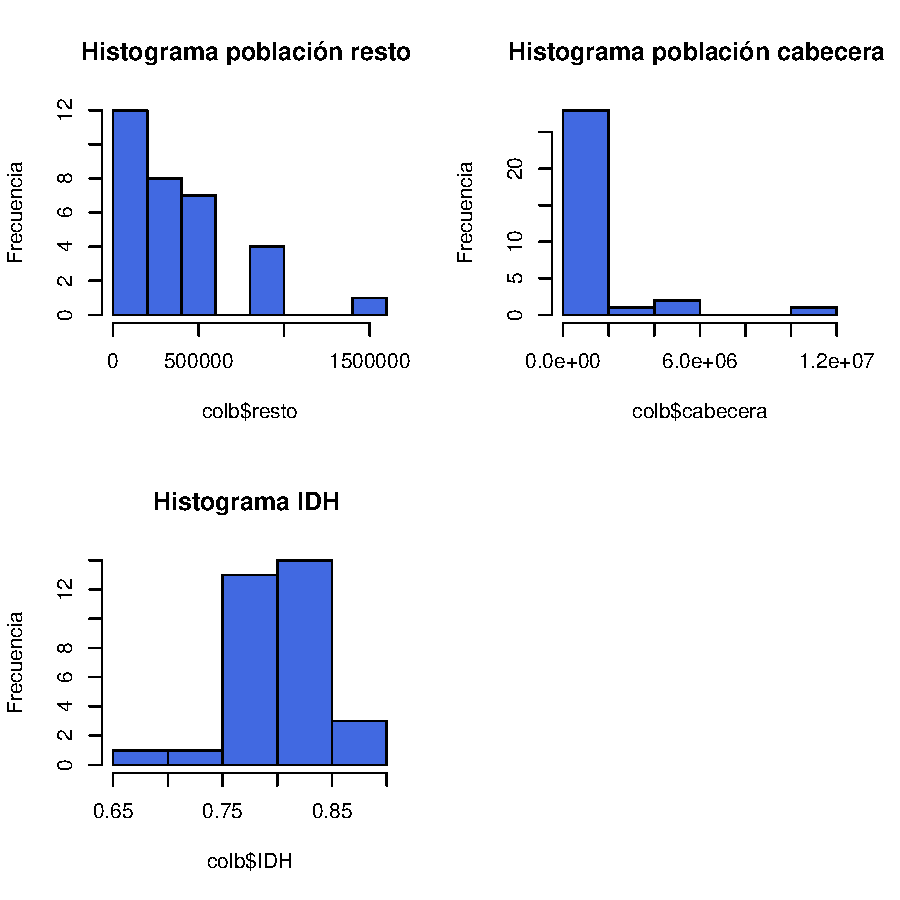
\includegraphics{Paper-histograma}
\caption{Histograma del IDH }
\label{histograma}
\end{figure}


Como las poblaciones tienen un sesgo se normalizan los datos con log, el histograma de estos nuevos datos se muestra en la Figura \ref{normal} en la página \pageref{normal}.

\begin{figure}[h]
\centering
\begin{adjustbox}{height=4cm}
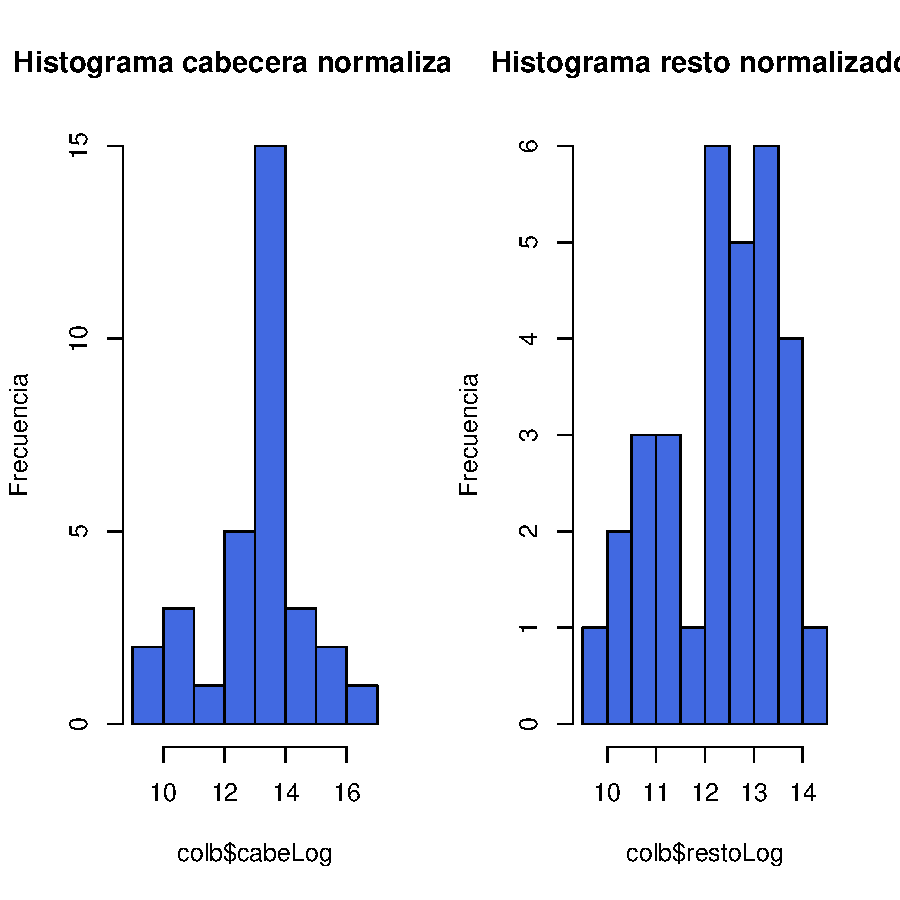
\includegraphics{Paper-normal}
\end{adjustbox}
\caption{Histograma de poblaciones }
\label{normal}
\end{figure}


\section{Exploración Bivariada}\label{bivariada}


en esta sección nos interesa ver el impacto que tiene la población en el IDH, para esto se presenta en la tabla ref{corrDem} en la página \pageref{corrDem}. la correlación de las variables normalizadas con respecto al IDH
¿+}


% Table created by stargazer v.5.2.2 by Marek Hlavac, Harvard University. E-mail: hlavac at fas.harvard.edu
% Date and time: mar, jul 03, 2018 - 05:49:52 p.m.
\begin{table}[!htbp] \centering 
  \caption{Correlación de Democracia con las demás variables} 
  \label{corrDem} 
\begin{tabular}{@{\extracolsep{5pt}} cc} 
\\[-1.8ex]\hline 
\hline \\[-1.8ex] 
total & cabeLog \\ 
\hline \\[-1.8ex] 
$0.399$ & $0.487$ \\ 
\hline \\[-1.8ex] 
\end{tabular} 
\end{table} 


Ademas, se muestra la correlacion entre todas las variables independientes en la tabla \ref{corrTableX} en la página \pageref{corrTableX}

% Table created by stargazer v.5.2.2 by Marek Hlavac, Harvard University. E-mail: hlavac at fas.harvard.edu
% Date and time: mar, jul 03, 2018 - 05:49:52 p.m.
\begin{table}[!htbp] \centering 
  \caption{Correlación entre variables independientes} 
  \label{corrTableX} 
\begin{tabular}{@{\extracolsep{5pt}} ccc} 
\\[-1.8ex]\hline 
\hline \\[-1.8ex] 
 & total & cabeLog \\ 
\hline \\[-1.8ex] 
total & 1 &  \\ 
cabeLog & 0.71 & 1 \\ 
\hline \\[-1.8ex] 
\end{tabular} 
\end{table} 
los datos anteriores los puede ver visualmente en la figura  \ref{puntos} en la página \pageref{puntos}

\begin{figure}[h]
\centering
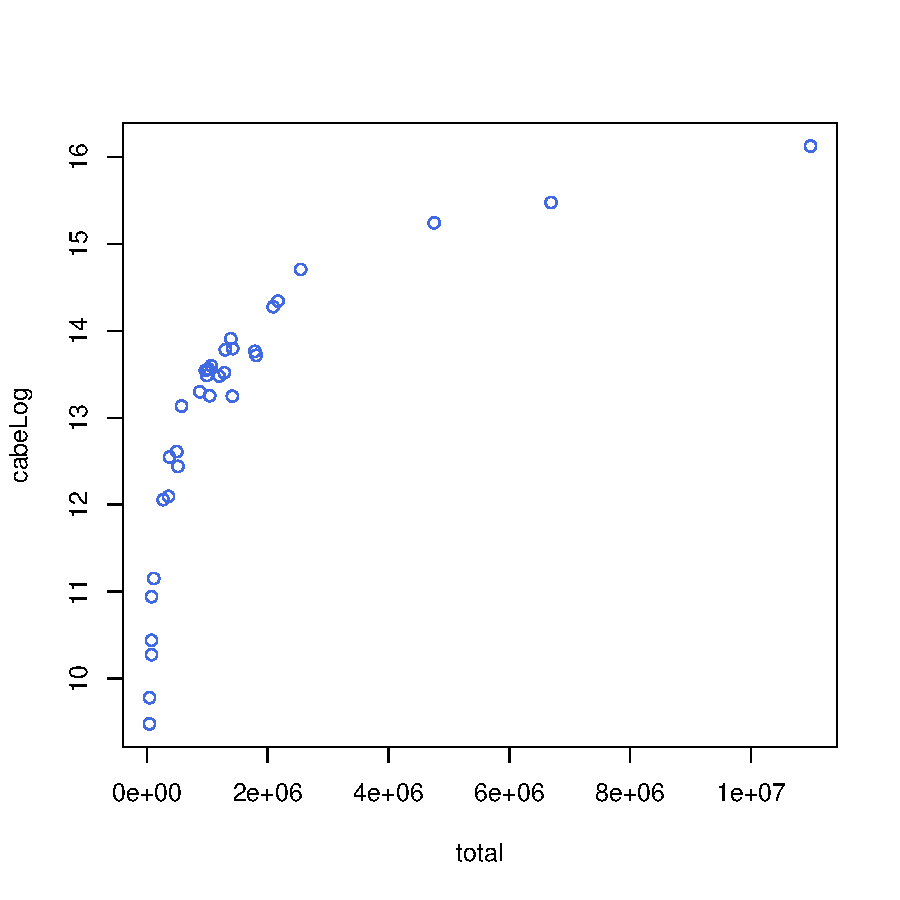
\includegraphics{Paper-puntos}
\caption{correlacion entre cabelog y restolog }
\label{puntos}
\end{figure}




\section{Modelos de Regresión}

Finalmente, vemos los modelos propuestos. En cada una se evalua la variable independiente DIH con cada una de las categorias de la poblacion. Los resultados se muestran en la Tabla \ref{regresiones} de la página \pageref{regresiones}.


% Table created by stargazer v.5.2.2 by Marek Hlavac, Harvard University. E-mail: hlavac at fas.harvard.edu
% Date and time: mar, jul 03, 2018 - 05:49:52 p.m.
\begin{table}[!htbp] \centering 
  \caption{Modelos de Regresión} 
  \label{regresiones} 
\begin{tabular}{@{\extracolsep{5pt}}lccc} 
\\[-1.8ex]\hline 
\hline \\[-1.8ex] 
 & \multicolumn{3}{c}{\textit{Dependent variable:}} \\ 
\cline{2-4} 
\\[-1.8ex] & \multicolumn{3}{c}{IDH} \\ 
\\[-1.8ex] & (1) & (2) & (3)\\ 
\hline \\[-1.8ex] 
 cabeLog & 0.013$^{***}$ &  &  \\ 
  & (0.004) &  &  \\ 
  & & & \\ 
 restoLog &  & 0.007 &  \\ 
  &  & (0.007) &  \\ 
  & & & \\ 
 totalLog &  &  & 0.013$^{**}$ \\ 
  &  &  & (0.005) \\ 
  & & & \\ 
 Constant & 0.634$^{***}$ & 0.722$^{***}$ & 0.629$^{***}$ \\ 
  & (0.055) & (0.082) & (0.068) \\ 
  & & & \\ 
\hline \\[-1.8ex] 
Observations & 32 & 32 & 32 \\ 
R$^{2}$ & 0.238 & 0.031 & 0.179 \\ 
Adjusted R$^{2}$ & 0.212 & $-$0.001 & 0.152 \\ 
Residual Std. Error (df = 30) & 0.037 & 0.042 & 0.039 \\ 
F Statistic (df = 1; 30) & 9.347$^{***}$ & 0.974 & 6.561$^{**}$ \\ 
\hline 
\hline \\[-1.8ex] 
\textit{Note:}  & \multicolumn{3}{r}{$^{*}$p$<$0.1; $^{**}$p$<$0.05; $^{***}$p$<$0.01} \\ 
\end{tabular} 
\end{table} 


















\endinput

\clearpage
\documentclass{article}

%%%%
% PLOTS mapas
% eval=FALSE
% results=HIDE (verbatim default)
%%%%
\usepackage[utf8]{inputenc}
\usepackage{longtable}
\usepackage{authblk}
\usepackage{adjustbox}

%%%%
\usepackage{Sweave}
\begin{document}
\Sconcordance{concordance:basico32departamentos.tex:basico32departamentos.Rnw:%
1 18 1 1 9 2 1 1 31 6 1 1 12 1 4 1 1 1 12 1 5 1 1 1 27 4 1 1 27 1 2 16 %
1}



%Partes extras para las nuevas columnas
% Exploracion Univariada --------------------------------------------------

\section{Exploración Espacial}

El siguiente mapa muestra el impacto que tiene la población de cada departamento sobre su respectivo IDH:





%con esto hagamos el merge:



 
 
\begin{figure}[h]
\centering
\begin{adjustbox}{width=8cm,height=6cm,clip,trim=1.5cm 2cm 0cm 2.5cm}
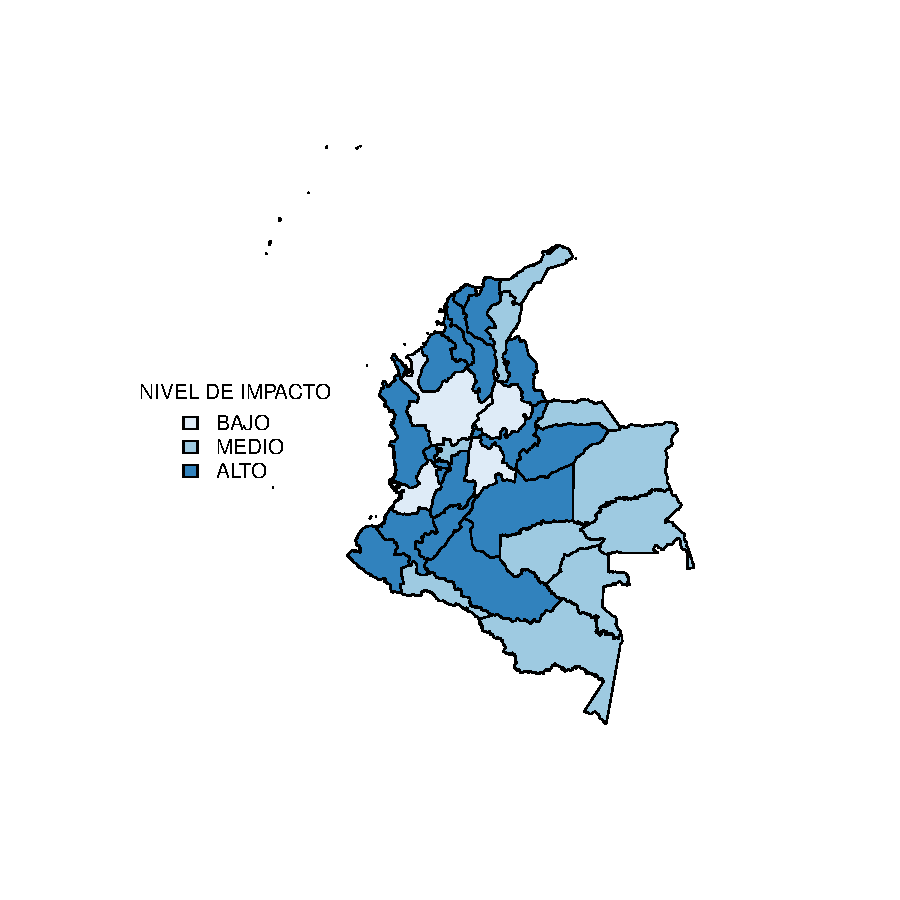
\includegraphics{basico32departamentos-plotMap0}
\end{adjustbox}
\caption{Impacto de población en IDH por departamento}\label{rawmap}
\end{figure}

Entre mayor es el impacto de la población sobre el IDH del departamento, más oscuro se muestra en el mapa. Se dividió el impacto en 3 niveles: BAJO, MEDIO Y ALTO.
Para lograr esta escala se implementó el siguiente procedimiento:

Primero se obtuvieron los datos de IDH, población de cabecera, el resto de la población y el total de la población de cada departamento del país.

Se limpiaron los datos reemplazando caracteres no reconocibles tales como la letra "ñ" y tildes.
Para evitar un sesgo significativo por variaciones amplias en número de habitantes, primero se utilizaron valores logarítmicos y luego se normalizaron. Finalmente se crearon las 3 agrupaciones por medio de la técnica K-means.





\end{document}




%\bibliographystyle{apalike}
%\renewcommand{\refname}{Bibliography}
%\bibliography{ProyectoHerramientas}

\end{document}
